\documentclass[russian, utf8]{eskdtext}
\newcommand*{\No}{\textnumero}
\ESKDdepartment{Кафедра Систем Управления и Информатики}
\ESKDcompany{Университет ИТМО}
\ESKDdocName{ПОЯСНИТЕЛЬНАЯ ЗАПИСКА}
\ESKDsignature{КСУИ.207.435.001 ПЗ}
\ESKDauthor{Овчаров А.О.}

\usepackage[hidelinks]{hyperref}

\usepackage{tocloft}
\renewcommand{\cftaftertoctitle}{\hfill}
\renewcommand{\cfttoctitlefont}{\hspace{7cm}\Large\bfseries}	%KOSTIL'
\renewcommand{\cftaftertoctitle}{\hfill}
\renewcommand{\cftdot}{.}
\renewcommand{\cftsecleader}{\cftdotfill{\cftdotsep}} % for sections
\makeatletter

\usepackage{wrapfig}
\usepackage{graphicx}
\graphicspath{{images/}}
\DeclareGraphicsExtensions{.pdf, .jpg, .png}

\usepackage{caption}
\captionsetup[table]{singlelinecheck=false}		% Заголовок таблиц слева
\captionsetup[table]{aboveskip=2pt,belowskip=2pt}			%belowskip=6pt 	% Позиционирование заголовка

\usepackage{tikz}

\begin{document}
\tableofcontents
\thispagestyle{empty}
\newpage

{\section*{Введение}
\addcontentsline{toc}{section}{Введение}}

Люди могли измерять плотность уже в древности. Так например Архимед в своем законе использует плотость жидкости. В настоящее время необходимость измерения плотности жидкости выросла до такой степени, что было выпущено множество статей и книг по способам и приборам измерения плотности. \par
\textbf{Плотностью} $\rho$ однородного вещества называют отношение его массы $m$ к объему $V$.
\begin{equation}
	\rho = \frac{m}{V}
\end{equation}
Для неоднородного вещества плотность определяется как предел отношения массы к объему, когда объем стягивается к точке, в которой определяется плотность:
\begin{equation}
	\rho = \lim_{\Delta V\rightarrow0}{\frac{\Delta m}{\Delta V}}
\end{equation}
где $\Delta m$ - масса элемеетраного объема $\Delta V$.

Также в ряде отраслей науки и техники для характеристики вещества применяю \textbf{относительную плотность}, представляющая собой отношение плотности рассматриваемого вещества к плотности другого, условного, вещества при определенных физических условиях. В качестве условного вещества обычно принимают дистилированную воду. \par

Существует достаточно много методов измерения плотности, на которых основана работа большого количества приборов. \par

Большую группу методов называют \textbf{поплавково-весовыми}, данные методы основаны на определении выталкивающей силы, действующее на испытуемое тело или вспомогательное тело (поплавок). Эта сила в соответствии с законом Архимеда прямо пропорциональная плотности среды, в которую погружено тело. Сюда можно отнести методы ареометра, гидростатического взвешивания, поплавковый, флотационный. \par

Следующую группу образуют \textbf{гидростатические} методы измерения, которые базируются на зависимости статического давления столба жидкости или газа постянной высоты от их плотности. \par

Выделяют также \textbf{гидродинамические} методы, основанные на зависимости от плотосни таких физических величин, как скорость истечения струи жидкости или газа из отверстия, сила удара струи о преграду, скорость падения тела в жидкости, энергия потока вещества, динамическое давление и др. \par

На сегодняшний день развились также и новые методы определения жидкости. \textbf{Радиационный} метод основан на зависимости плотности от ослабления радиоактивного излучения облученного вещества. \textbf{Ультразвуковой} метод основан на скорости распронения ультразвуковых волн в веществе. \textbf{Вибрационный} метод основан на зависимотси плотности от параметров упругих колебаний, сообщаемых сусуду с исследуемым веществом. \par

Приборы, осуществляющие измерение плотности называются \textbf{плотномерами}. Далее будут рассмотрены плотномеры, работающие по разным принципам.

\newpage

\section{Попавковый плотномер}

Действие поплавковых плотномеров основано на зависимости плотности от перемещения поплавка от нейтрального положения или наоборот, перемещения жедкости при неподвижном поплавке. \par

На рисунке 1 представлена схема плотномера с плавающим поплавком. Жидкость по трубке 6 поступает в переливной сосуд 5, а оттуда по проводящей трубке 4 поступает в измерительный сосуд 2, который также снабжен переливным устройством. Требуемая скорость потока устанавливается диафрагмой 10. Для отвода излишков воды имеется трубка 9. В результате действия выталкивающей силы поплавок перемещается по вертикали, тем самым сердечник совершает те же перемещения вдоль индуктивного датчика 7, включенный в схему измерительного моста 1. Для коррекции показаний изменение температуры, используется датчик температуры 3. \par 

\begin{figure}[h!]
	\centering
	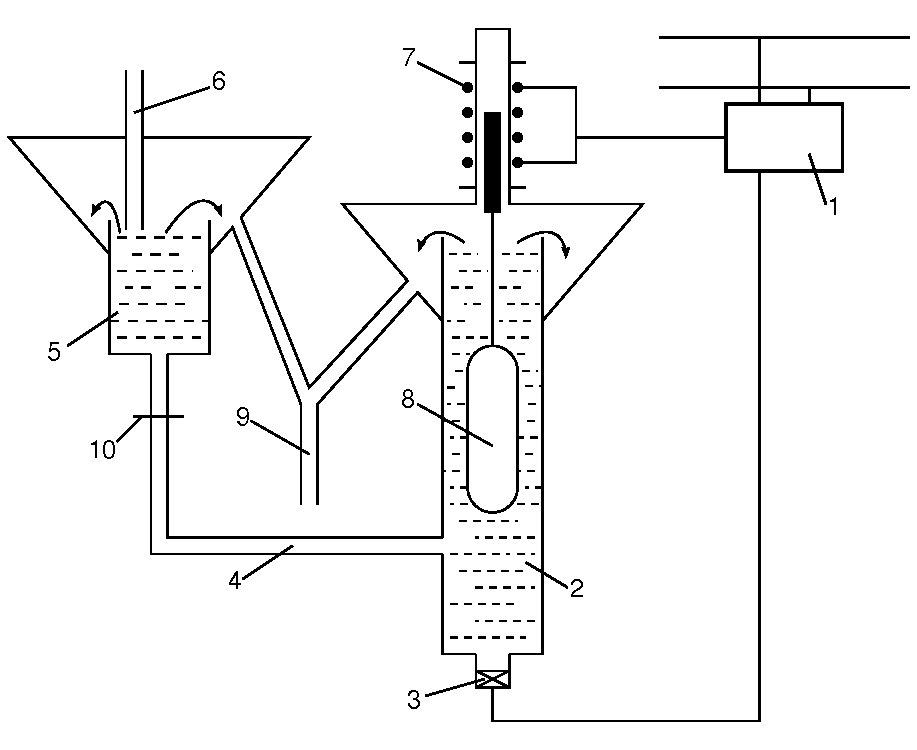
\includegraphics[width = 0.7\textwidth] {FloatDensityMeter.pdf}
	\caption{Схема плотнометра с плавающим поплавком}
\end{figure}

\newpage

На поплавок действует выталкивающая сила по закону Архимеда, эта сила компенсирует вес тела поплавка и вес миниска. В силу малости выталкивающей силы миниска в воздухе, она не учитывается. Таким образом сила Архимеда включает в себя две части:

\begin{align}
	P_a & = (v + lS)\rho g \\
	P_c & = (V - v - lS)D
\end{align}
где выражение (1) характерезует вес жидкости в обхеме погруженной части стержня, а выражение (2) вес воздуха в обхеме погруженно части стержня. \par

Тогда можем записать закон архимеда, с учетом того, что поплавок не тонет: 
\begin{equation}
	m + La\rho = (v + lS)\rho + (V - v - lS)D
\end{equation}
или
\begin{equation}
	m - VD + La\rho = (v + lS)\rho - (v + lS)D
\end{equation}
здесть $v$ - объем нижней части поплавка без стержня; $l$ - длинна погруженно части стержня; $L$ - длинна окружности сечения стержня; $M$ - масса поплавка в воздухе; $m$ - масса поплавка; $D$ - плотность воздуха; $a$ - капилярная постоянная. Выражение $La\rho$ характеризует массу миниска, обвалакивающего стержень. \par 

Учитывая, что $m - VD$ есть масса $M$ поплавка в воздухе, получим итоговое выражение для плотности.

\begin{equation}
	\rho = \frac{M + (v + lS)D}{v + lS - La}
\end{equation}

Объем попловка определяютс из пределов цены деления шкалы прибора. \par

Данный прибор имеет довольно простую и не дорогостоющую конструкцию, при том он позволяет измерять плотность с большой точностью (0.2 - 2\%) и с учетом температурных изменений. Также прибор долвольно интертный, из-за чего процесс измерения плотности становится довольно длительным. 

\newpage

\section{Гидростатический плотномер}

Гидростатический метод измерения плотности основан на зависимости давления $P$ столба жидкости высотой $H$ от плотности $\rho$ жидкости. Эта завсисимость определяется формулой:
\begin{equation}
	P = \rho g H
\end{equation}

Но на практике, чтобы ислкючить влияние колебаний уровня жидкости, применяют дифференциальный метод при измерении разности давлений $\Delta P$ двух столбов жидкости разной высоты: 
\begin{equation}
	\Delta P = \rho g h 
\end{equation}
где $h$ - разность высот столбов жидкости. \par

Давайте рассотрим патент RU 2 589 773 C1. Ниже, на рисунке 2, представлен разработанные прибор измеряющий расход и плотность пульпы в напорных трубопроводах. 

\begin{figure}[h!]
	\centering
	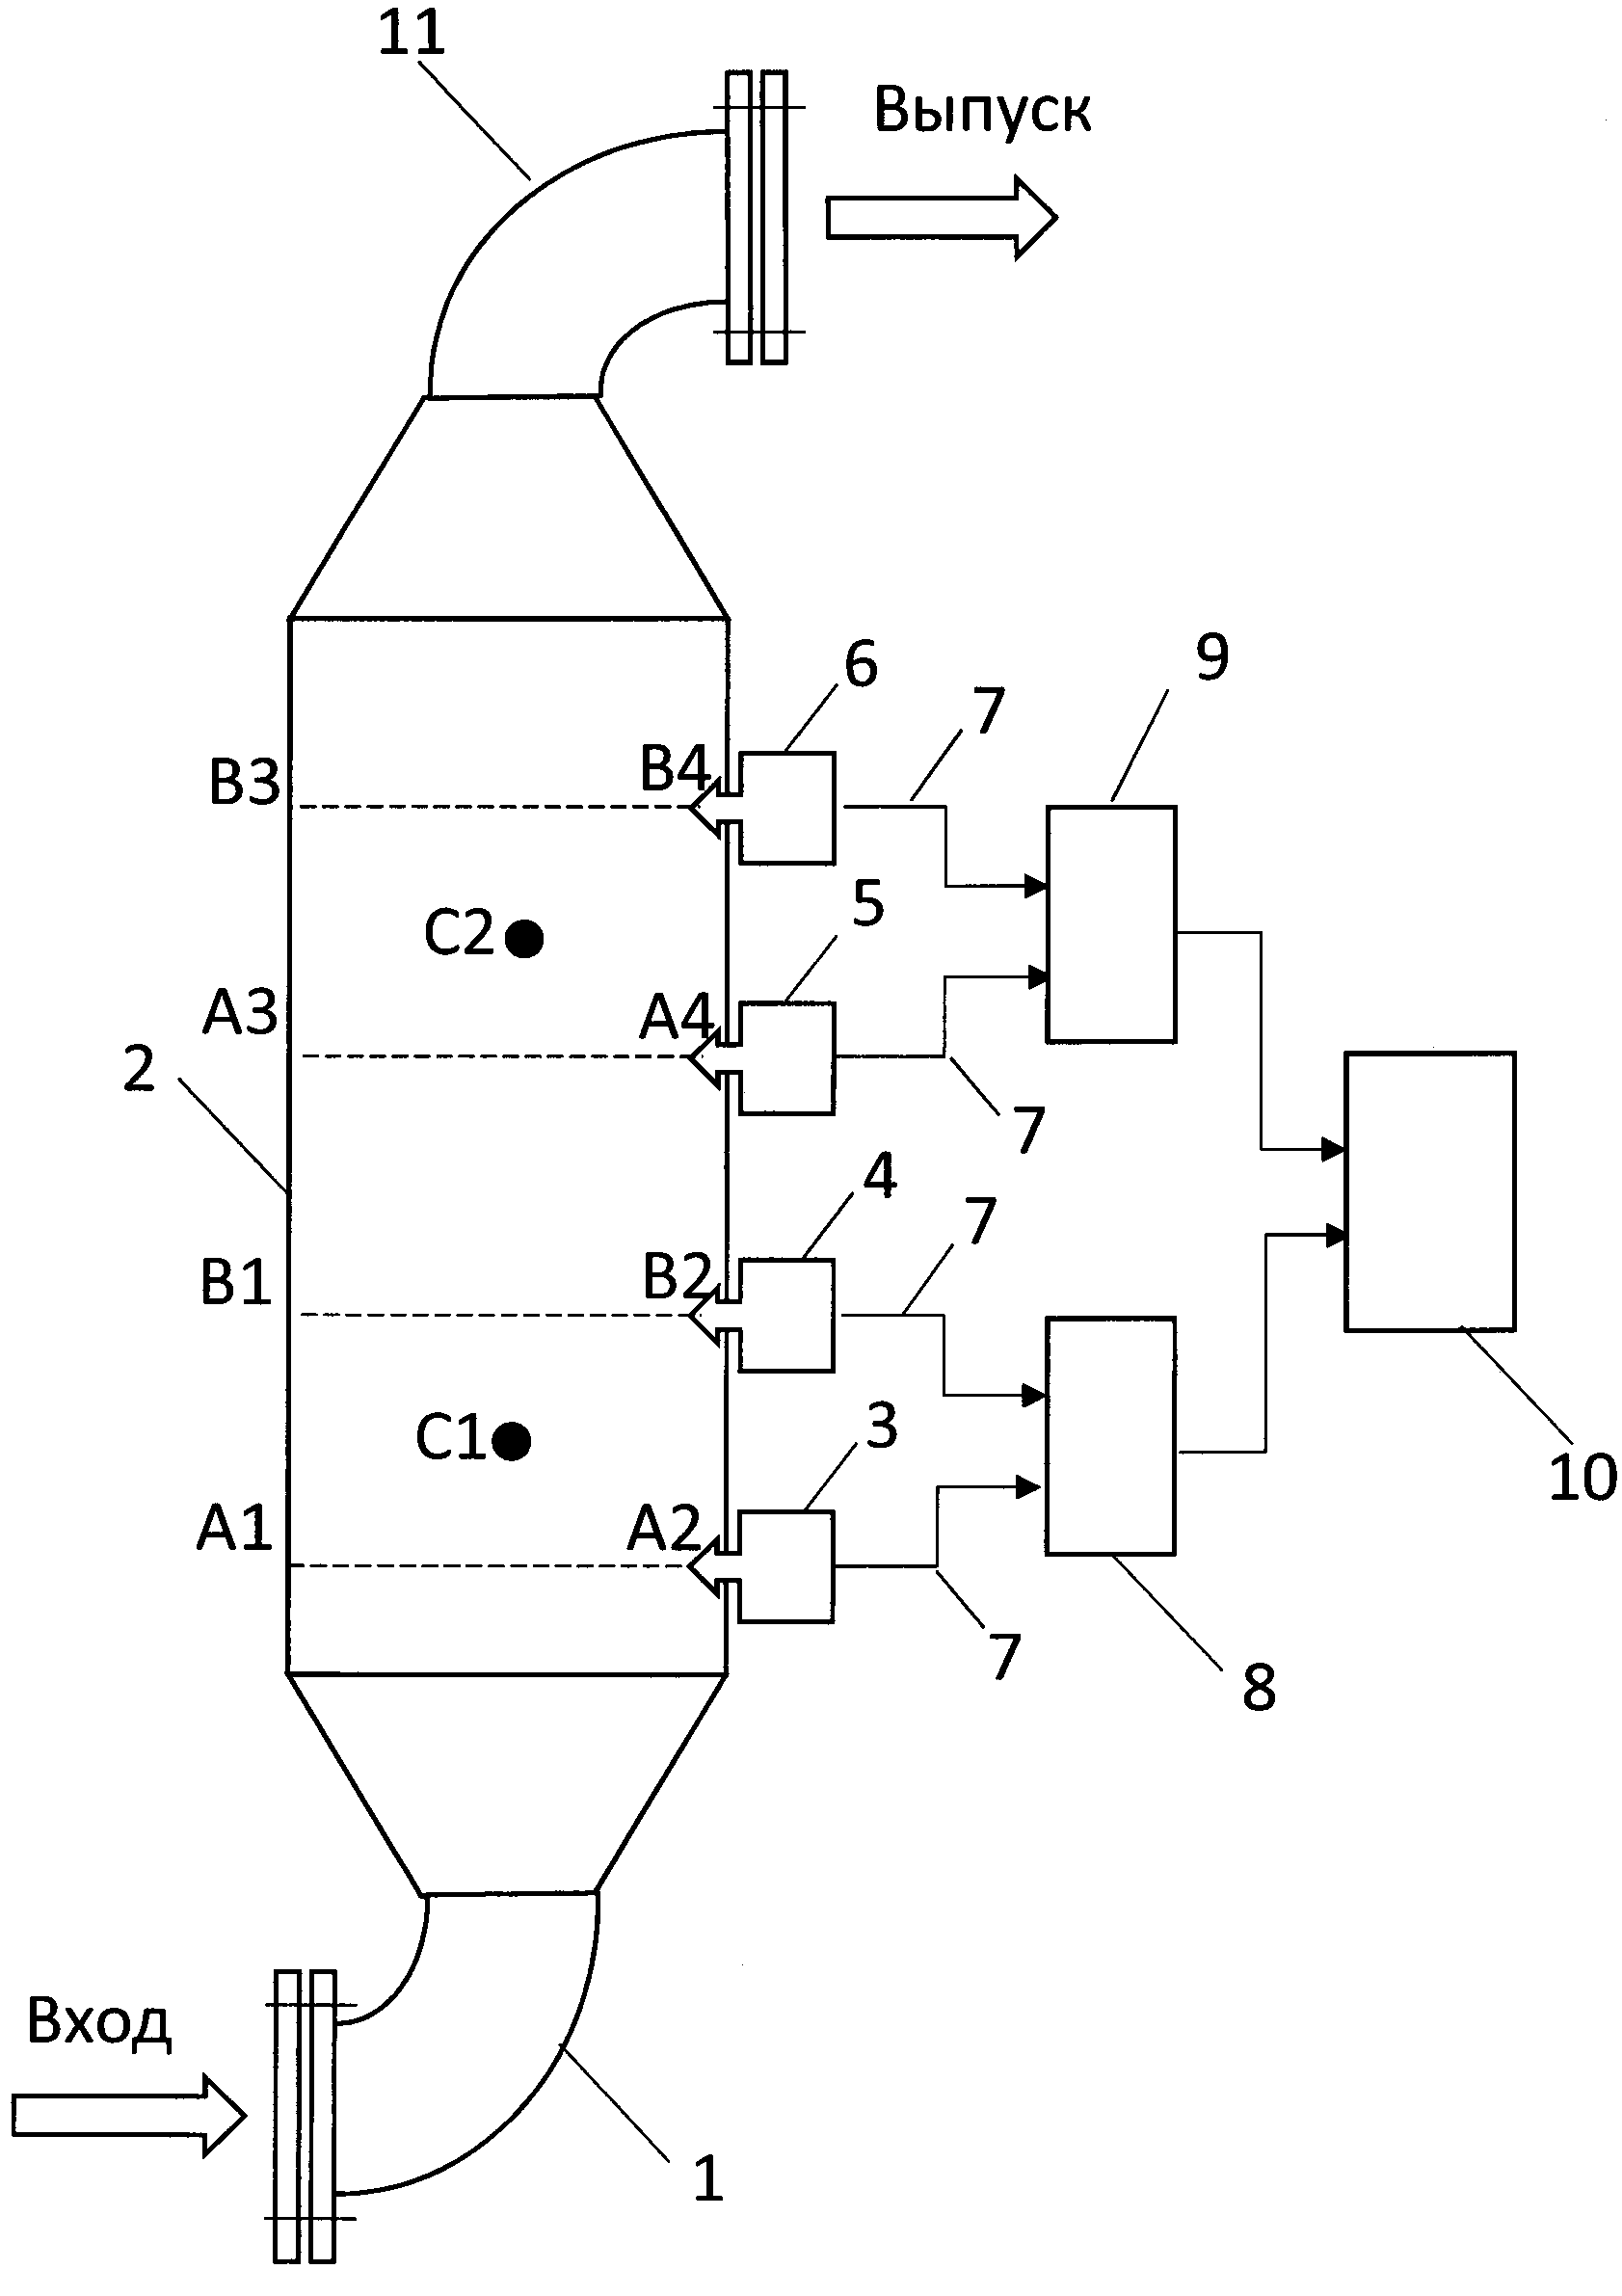
\includegraphics[width = 0.4\textwidth] {HydrostaticDensityMeter.png}
	\caption{Устройство для измерения плотности и расхода жидкости}
\end{figure}

\newpage
Данное устройство содержит впускной патрубок 1, напорный трубопровод 2, устройства 3, 4, 5 и 6 отбора давления, импульсные линии 7, датчики перепада давления 8 и 9, вычислительное устройство 10, выпускной патрубок 11. \par

Измерив при помощи датчиков давления 3 - 6 мы можем найти разность давления:
\begin{align}
	\Delta P_1 & = P_2 - P_1 \\
	\Delta P_2 & = P_4 - P_3
\end{align}
где $P_1$ и $P_2$ - величины давлений пульпы, измеренных на нижней и верхней границах 1-го участка; $\Delta P_1$ - величина перепада давления на первом участке. Аналогично для второго участка. \par

Теперь воспользовавшись выражением (9) можем найти значение плотности данной жидкости.

\begin{equation}
	\rho = \frac{\Delta P_1}{gh}
\end{equation}

Хочется также дополнить, что расстояние моежду двумя точками измерения давления определяется из пределов измерения плотности и давления: 

\begin{equation}
	\begin{cases}
		\Delta P_{max} = gh \rho_{max} \\
		\Delta P_{min} = gh \rho_{min}
	\end{cases}
\end{equation}

Данный прибор обладает высокой погрешностью - $\pm 1$\% диапозона шкалы. Такими плотномерами можно измерять плотность вязких, загрязненных, кристаллизирующихся и агрессивных жедкостей, они пригодны как для открытых, так и для закрытых резервуаров. Их показания не зависят от скорости потока жидкости и ее поверхностного натяжения. \par

Из недостатков хочется отметить, что для высокой точности требуется большая высота столба, что делает прибор довольно громоздким.

\newpage

\section{Вибрационный плотномер}

На рисунке 3 представлена упрощенная схема вибрационного плотномера. Данный прибор относится к частотному типу вибрационных плотномеров, в которых измеряют функционально связанную с плотностью вещества частоту собственных колебаний резонатора.
\begin{figure}[h!]
	\centering
	\begin{tikzpicture}
		%\draw[gray, dashed] (0, 0) grid (15, 6);
		\draw (7, 3) node {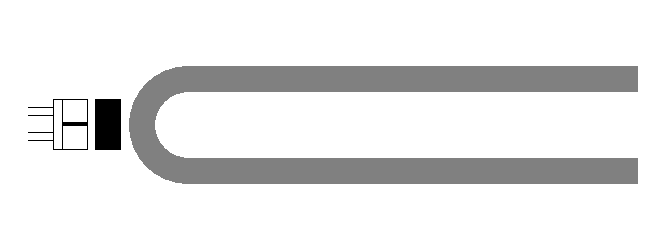
\includegraphics {VibratingDensityMeter.pdf}};
		\draw[thick, ->] (3.1, 5.1) -- (3.1, 3.45); \draw (3.1, 5.1) node[anchor = south] {Магнит};
		\draw (12.5, 3) node {Измерительная трубка};
		\draw[thick, ->] (2.7, 1.5) -- (2.7, 2.6); \draw (1.5, 1.5) node[anchor = north west] {Контроллер колебаний/измеритель колебаний};
	\end{tikzpicture}
	\caption{Упрощенная схема плотномера DE40/DE45}
\end{figure}

Здесь контроллер колебаний, преставляющий собой катушку инуктивности с переменным напряжением определенной частоты, изменение магнитного поля катушки заставляет магнит, то отталкиваться, то притягиваться, что вызывает колебания измерительно трубки с измеряемой жидкостью. \par

Период колебаний $T$ системы определяется следующим выражением:
\begin{equation}
	T = 2\pi \sqrt{\frac{\rho V_c + m_c}{K}}
\end{equation}
здесь $\rho$ - плотность содержимого трубки, $V_c$ - объем внутренней части трубки, $m_c$ - масса трубки, $K$ - коэффициент жесткосит трубки. \par

Теперь можем получить вырежение для плотости: 
\begin{equation*}
	\rho = \frac{K}{4\pi^2 V_c}T^2 - \frac{m_c}{V_c} = AT^2 + B
\end{equation*}

Далее измерения можно упростить, введя $\rho_W$ - плотность воды, $\rho_A$ - плотность воздуха. Найдем их разность, полюзуясь выражением (15), получим:
\begin{equation*}
	\rho_A - \rho_W = A(T_A^2 - T_W^2)
\end{equation*}

Тогда можем найти коэффициент $A$:

\begin{equation*}
	A = \frac{\rho_A - \rho_W}{T_A^2 - T_W^2}
\end{equation*}
данную процедуру также называют калибровкой плотномера.

И поскольку плостность воздуха $\rho_A$ ялвяется табличной величиной, его можно использовать при измерении искомой плотности жидкости $\rho_S$.

\begin{equation*}
	A(T_A^2 - T_S^2) = \rho_A - \rho_S
\end{equation*}

В итоге получим искомое значение плотности жидкости:
\begin{equation}
	\rho_S = \rho_A - A(T_A^2 - T_S^2)
\end{equation}

Как видно из выражения (15) пределы измерения зависит от жесткости и объема трубки, а также от частоты колебаний контроллера. \par
Основным достоинством данных плотномеров является выскокая точность, чувствительность и надежность. \par
Вместе с тем частотные плотномеры обладают и недостатками, к которым относятся ограниченность допускаемого расзода вещества определяемого площадью сечения канала, нелинейность шкалы.

\newpage

\section{Ультразвуковой плотномер}

\end{document}